%---------------------------------------------------------------------
%
%                          Ap�ndice UML
%       Para poner las im�genes de los dise�os UML
%
%---------------------------------------------------------------------

\chapter{Diagramas de dise�o de PMCTrack-GUI}
\label{app:UML}


%\begin{resumen}
En este ap�ndice incluimos los diagramas que hemos usado durante el dise�o de nuestra aplicaci�n PMCTrack-GUI, y que sin duda, servir�n al lector para un mayor entendimiento de la aplicaci�n. Las dos primeras secciones de este ap�ndice constan de diagramas UML que representan el modelo de objetos actual de alguno de los componentes de PMCTrack-GUI. En la tercera secci�n se muestran los primeros bocetos o *mockups* que se desarrollaron sobre la interfaz gr�fica de PMCTrack-GUI.
%\end{resumen}

\clearpage

\begin{landscape}

%-------------------------------------------------------------------
\section{Diagrama UML: Objetos de procesamiento}
%-------------------------------------------------------------------
\label{app:UML.XML}
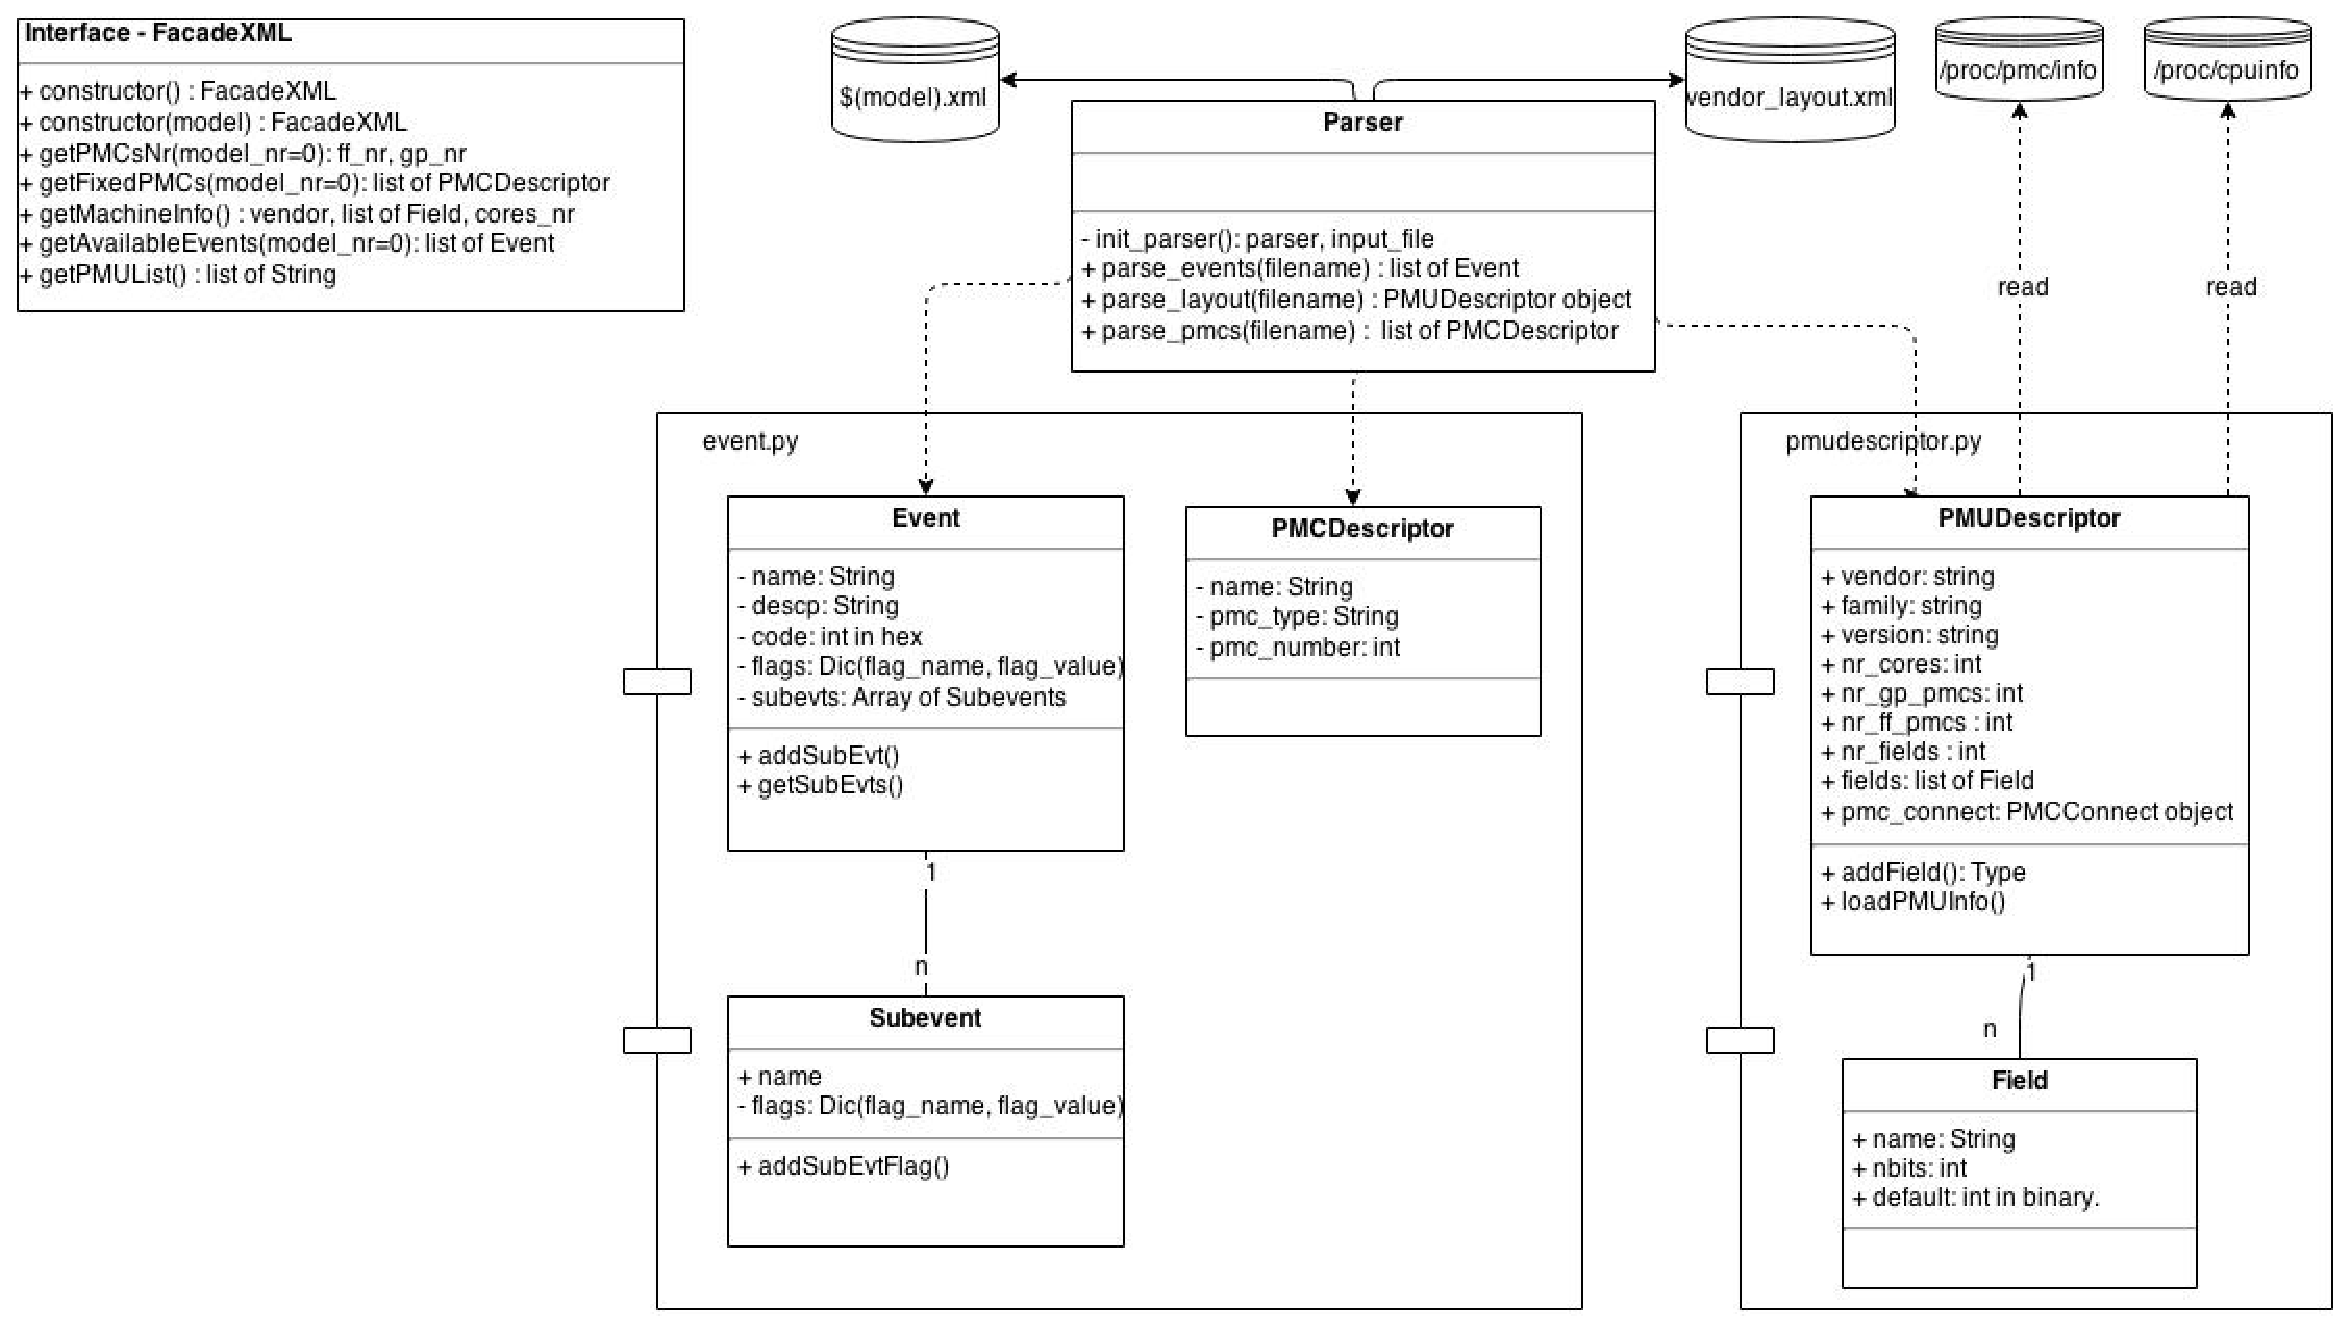
\includegraphics[scale=0.5]{Imagenes/Bitmap/XMLdiagram}

%-------------------------------------------------------------------
\section{Diagrama UML: Objetos de configuraci�n de usuario}
%-------------------------------------------------------------------
\label{app:UML.UserConfig}
\includegraphics[scale=0.5]{Imagenes/Bitmap/UserConfigDiagram}

%-------------------------------------------------------------------
\section{Primeros bocetos de la interfaz gr�fica}
%-------------------------------------------------------------------
\label{app:Bocetos}
\includegraphics[scale=0.5]{Imagenes/Bitmap/Select_Event_1}
\includegraphics[scale=0.5]{Imagenes/Bitmap/Select_Event_2}
\includegraphics[scale=0.5]{Imagenes/Bitmap/Select_Event_3}
\includegraphics[scale=0.5]{Imagenes/Bitmap/Select_Event_4}

\end{landscape}
